\documentclass[journal]{IEEEtran}

\usepackage[T1]{fontenc}
\usepackage[utf8]{inputenc}
\usepackage{amsmath,amssymb,amsfonts}
\usepackage{graphicx}
\usepackage{booktabs}
\usepackage{array}
\usepackage{url}
\usepackage{xcolor}
\usepackage[hidelinks]{hyperref}
\usepackage{orcidlink}
\usepackage{balance}

\graphicspath{{../figures/}}

\renewcommand{\topfraction}{0.92}
\renewcommand{\bottomfraction}{0.75}
\renewcommand{\textfraction}{0.08}
\renewcommand{\floatpagefraction}{0.80}

% IEEEtran hard-codes an em-dash after the abstract and index-terms names; the CAOS
% content standard (ADR-0067) excludes em-dashes, so the separator is a full stop.
\makeatletter
\def\abstract{\normalfont
    \if@twocolumn
      \@IEEEabskeysecsize\bfseries\textit{\abstractname}.\ \relax
    \else
      \bgroup\par\addvspace{0.5\baselineskip}\centering\vspace{-1.78ex}\@IEEEabskeysecsize\textbf{\abstractname}\par\addvspace{0.5\baselineskip}\egroup\quotation\@IEEEabskeysecsize
    \fi\@IEEEgobbleleadPARNLSP}
\def\IEEEkeywords{\normalfont
    \if@twocolumn
      \@IEEEabskeysecsize\bfseries\textit{\IEEEkeywordsname}.\ \relax
    \else
      \bgroup\par\addvspace{0.5\baselineskip}\centering\@IEEEabskeysecsize\textbf{\IEEEkeywordsname}\par\addvspace{0.5\baselineskip}\egroup\quotation\@IEEEabskeysecsize
    \fi\@IEEEgobbleleadPARNLSP}
\makeatother

% Page-1 header block (conventions/manuscript-header-standard.md). The four document
% macros are set by the publishing tool when the version DOI is reserved.
\newcommand{\doctype}{Technical report}
\newcommand{\docversion}{v1.1}
\newcommand{\docdate}{18 September 2026}
\newcommand{\versiondoi}{10.5281/zenodo.22824572}
\newcommand{\conceptdoi}{10.5281/zenodo.21519229}
\newcommand{\docrepo}{github.com/fsantibanezleal/CAOS\_CoreLog}
\newcommand{\headerblock}{%
\begin{center}
\fbox{\parbox{0.94\textwidth}{\small\raggedright
\textbf{\doctype} \quad$\cdot$\quad \docversion, \docdate \quad$\cdot$\quad Licence CC BY 4.0\\[2pt]
CAOS open-research programme \quad$\cdot$\quad CAOS\_CoreLog, lithology from drill-core imagery\\[2pt]
Version DOI \href{https://doi.org/\versiondoi}{\texttt{\versiondoi}} \quad$\cdot$\quad
concept DOI (always latest) \href{https://doi.org/\conceptdoi}{\texttt{\conceptdoi}}\\[2pt]
Not peer reviewed. Source code, data and computational records: \href{https://\docrepo}{\texttt{\docrepo}}
}}
\end{center}}

\begin{document}

\title{CoreLog Vision: Lithology from\\ Drill-Core Imagery, with Sim-to-Real\\ Out-of-Distribution Detection}

\author{Felipe~Santiba\~nez-Leal~\orcidlink{0000-0002-0150-3246}%
\thanks{F. Santiba\~nez-Leal is with the CAOS open-research programme, Santiago, Chile
(e-mail: fsantibanez@gmail.com; ORCID 0000-0002-0150-3246).}%
\thanks{Interactive tool and reproducible pipeline (MIT) at
\url{https://github.com/fsantibanezleal/CAOS_CoreLog}; the tool is available at
\url{https://corelog.fasl-work.com}.}}

% The leading {} lets IEEEtran's \MakeUppercase reach \doctype, so the whole head is set in capitals.
\markboth{{}\doctype\ \docversion, 2026}%
{Santiba\~nez-Leal: Lithology from drill-core imagery with sim-to-real OOD detection}

\IEEEaftertitletext{\vspace{-0.6\baselineskip}\headerblock\vspace{0.2\baselineskip}}

\maketitle

\begin{abstract}
Logging the lithology of drill core, identifying the rock type down a borehole from the core in its trays, is slow
and subjective manual work, and automating it from core-tray photographs is a natural target for computer vision.
Labelled core photographs are scarce, so a model is often trained on synthetic core or on one operation's core and
then applied to another's, where it answers confidently and wrongly unless it can tell that the new core is unlike
its training data. CoreLog Vision classifies core-tray imagery into lithologies and detects core that lies outside
its training distribution. On synthetic core a small convolutional network reaches $99.4\%$ accuracy over six
lithologies, against $92.9\%$ for a colour-and-texture baseline, on a split that holds out entire boreholes. On real
core from the open DCID-7 drill-core image dataset, a linear head over frozen ImageNet MobileNetV3-Small features
reaches $99.2\%$ over seven lithologies, and a linear head over the features of the synthetic-trained network
reaches $88.8\%$; the two heads differ in backbone and in input resolution, so the difference does not isolate the
cost of synthetic training. Nine out-of-distribution detectors are benchmarked at separating real DCID-7 core from
held-out synthetic core, with both streams reduced to the same $24$-pixel window. Distance detectors in a network's
feature space reach an area under the precision-recall curve (AUPR) of $0.92$ to $0.999$, softmax-based scores
$0.74$ to $0.83$, and the reconstruction error of an autoencoder ranks the two populations in the wrong order
(AUPR $0.28$, below the chance level of $0.38$). Distance in a feature space detects this shift; reconstruction
error does not.
\end{abstract}

\begin{IEEEkeywords}
Drill-core logging, lithology classification, computer vision, convolutional neural networks, out-of-distribution
detection, sim-to-real, Mahalanobis distance, mineral exploration, distribution shift.
\end{IEEEkeywords}

\section{Introduction}

\IEEEPARstart{A} geologist logs a drill hole by reading its core, tray by tray, and naming the rock type at each
depth, a task that is slow, tiring and subjective, and that produces the lithology column every downstream
mine-planning decision rests on. Photographs of the core trays are routinely taken, so classifying lithology from
those images with computer vision is a natural automation, and convolutional networks do it
well~\cite{krizhevsky,he,alzubaidi,fu}. The obstacle is the data. Labelled core imagery is scarce and
operation-specific: core from one deposit, one drill and one photographic setup looks different from another's, so a
model trained on synthetic core or on one mine's photographs faces a distribution shift when applied elsewhere. A
classifier answers confidently on such out-of-distribution core and can be wrong without any sign of it, which in a
logging context means a corrupted lithology column that no one flagged.

CoreLog Vision segments a core-tray image along each core channel, classifies each window's lithology with a small
convolutional network run in the browser, and stitches a depth log. Two further elements address the problem above.
The classifier is evaluated on a split that holds out entire boreholes, so the accuracy is that of a new hole rather
than of patches from holes seen in training. And an out-of-distribution detector flags incoming core that is unlike
the training data. The classifier is evaluated on synthetic and on real core, and nine detectors are benchmarked on
the sim-to-real shift.

\section{The Lithology Classifier}\label{sec:cnn}

\begin{figure*}[!t]
\centering
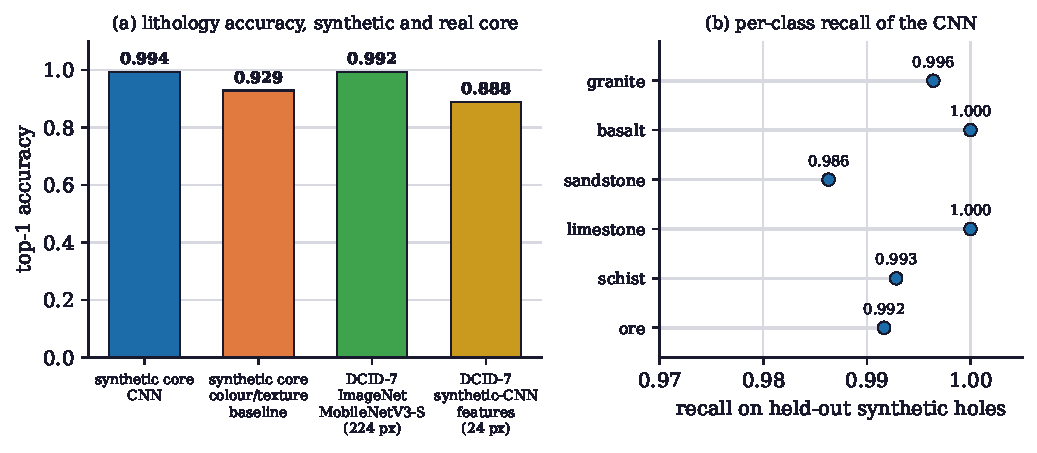
\includegraphics[width=0.86\textwidth]{fig-litho.pdf}
\caption{Lithology classification accuracy. \textbf{(a)} On synthetic core the convolutional network reaches
$99.4\%$ against $92.9\%$ for a colour-and-texture baseline, on a split that holds out entire boreholes. On real
DCID-7 core, a linear head over frozen ImageNet MobileNetV3-Small features (224-pixel input) reaches $99.2\%$ over
seven lithologies, and a linear head over the 64-dimensional features of the synthetic-trained network (24-pixel
input) reaches $88.8\%$. \textbf{(b)} Per-class recall of the network on the held-out synthetic holes: $0.986$ to
$1.000$ across the six lithologies.}
\label{fig:litho}
\end{figure*}

The classifier is a small convolutional network, two convolutional layers of $16$ and $32$ channels with max
pooling, a $64$-unit feature layer and a six-way softmax, applied to $24\times24$-pixel RGB windows along each core
channel. It is trained on procedurally generated core in six lithologies (granite, basalt, sandstone, limestone,
schist and ore) and runs in the browser. Its accuracy is measured on a split that holds out entire boreholes, $14$
holes for training ($4704$ windows) and $4$ for testing ($1344$ windows), so no window from a test hole is seen in
training; random patch splits inflate core-logging accuracy by letting near-identical patches of one hole appear on
both sides. On this split (Fig.~\ref{fig:litho}) the network reaches $99.4\%$ accuracy, against $92.9\%$ for a
nearest-centroid classifier on colour and texture features evaluated on the same windows, a margin of $6.5$
percentage points. Its per-class recall lies between $0.986$ (sandstone) and $1.000$ (basalt, limestone).

\section{Real Core and the Sim-to-Real Gap}\label{sec:real}

The real core comes from the open drill-core image dataset DCID~\cite{dcid}, in its seven-class form DCID-7 (red
sandstone, light sandstone, gray siltstone, mudstone, granite, basalt and marble): a class-balanced subset of the
dataset's own train and test split, with perceptual-hash deduplication across the split ($2062$ training and $829$
test images). Two linear
classification heads are trained on the real training images over frozen features (Fig.~\ref{fig:litho}a). Over the
features of an ImageNet-pretrained MobileNetV3-Small~\cite{howard} at $224$-pixel input, the head reaches $99.2\%$
top-1 accuracy on the test images (macro-F1 $0.992$). Over the $64$-dimensional features of the network trained on
synthetic core, with each image reduced to the $24$-pixel window that network reads, the head reaches $88.8\%$
(macro-F1 $0.887$). With permuted training labels the MobileNetV3-Small head falls to chance ($0.139$, against
$1/7=0.143$). Real core is
therefore learnable to high accuracy from real labels. The $10.4$-point difference between the two heads combines
two changes, the backbone and the input resolution, and the runs do not separate them, so it bounds the combined
effect rather than measuring the cost of synthetic training alone.

\section{Detecting Out-of-Distribution Core}\label{sec:ood}

\begin{figure*}[!t]
\centering
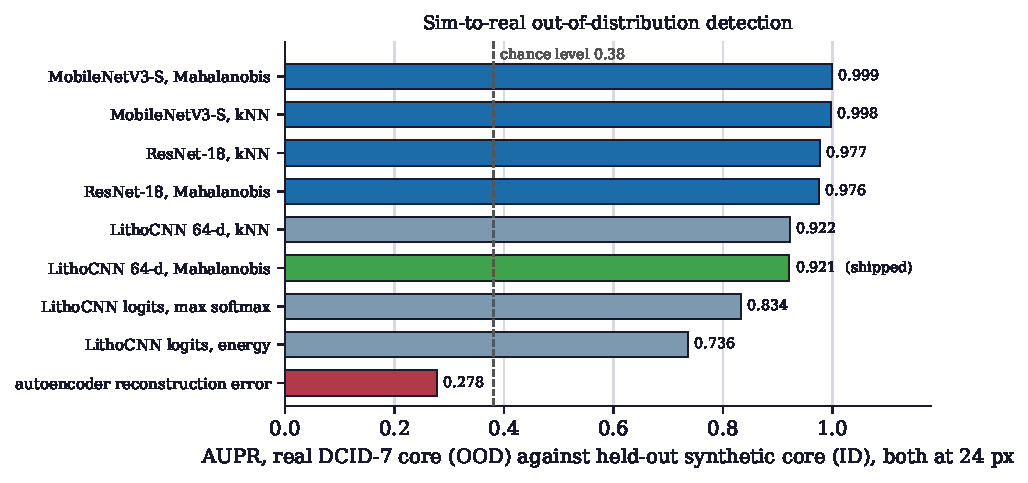
\includegraphics[width=0.76\textwidth]{fig-ood.pdf}
\caption{Sim-to-real out-of-distribution detection: nine detectors separating real DCID-7 core (out of
distribution, $829$ windows) from held-out synthetic core (in distribution, $1344$ windows), scored by the area
under the precision-recall curve (AUPR). Both streams are reduced to the same $24$-pixel window. The dashed line is
the chance level, the out-of-distribution fraction $0.38$. Distance detectors in a network's feature space reach
$0.92$ to $0.999$, the softmax-based scores $0.74$ to $0.83$, and the autoencoder's reconstruction error falls below
chance ($0.28$).}
\label{fig:ood}
\end{figure*}

The guard against silent sim-to-real error is an out-of-distribution detector (Fig.~\ref{fig:ood}). Nine detectors
are benchmarked on separating real DCID-7 core (out of distribution) from held-out synthetic core (in distribution),
with a control against a trivial cue: both streams are reduced to the same $24$-pixel window the classifier reads,
so no detector can separate them by raw resolution or sharpness alone. The distance detectors work in a network's
feature space, as the Mahalanobis distance to the nearest class mean under a shared covariance~\cite{lee} or as the
distance to the $k$-th
nearest neighbour ($k=10$) among normalised training features~\cite{sun}. In the frozen ImageNet features of
MobileNetV3-Small and ResNet-18~\cite{he}, with the $24$-pixel windows upsampled to the backbones' input size, they
reach AUPR $0.976$ to $0.999$; the best, the Mahalanobis distance in MobileNetV3-Small features, reaches $0.999$
(AUROC $0.9995$) and flags $0.2\%$ of the synthetic windows at $95\%$ recall of the real ones. In the classifier's own
$64$-dimensional features they reach $0.92$ (Mahalanobis: AUROC $0.95$, with $28\%$ of synthetic windows flagged at
$95\%$ recall); this detector reuses the classifier's features and is the one the tool runs. The maximum softmax
probability~\cite{hendrycks} and the energy score~\cite{liu} of the classifier reach $0.83$ and $0.74$. The
reconstruction error of a patch autoencoder trained on synthetic core fails: its AUROC of $0.31$ means that real
core reconstructs with lower error than held-out synthetic core, so the score ranks the two populations in the wrong
order, and its AUPR of $0.28$ lies below the chance level of $0.38$. To detect that incoming core is unlike the
training data, distance in a feature space works on this shift and reconstruction error does not.

\section{Discussion and Scope}\label{sec:discuss}

On synthetic core the classifier reaches $99.4\%$ and exceeds the colour-and-texture baseline; on real core a linear
head reaches $99.2\%$ over ImageNet features and $88.8\%$ over the features of the synthetic-trained network; and the
real core is separated from the synthetic training core at AUPR up to $0.999$ in a feature space, while
reconstruction error fails. The measurements have limits. The six-class accuracy is measured on procedurally
generated core, which allows controlled evaluation but is not a photograph of real rock. The real-core numbers come
from one open dataset, and a deployment would need labels from the target operation. The two real-core heads differ
in backbone and input resolution, so their difference is not a clean measure of the sim-to-real gap. The
out-of-distribution benchmark tests one large shift, from synthetic to photographed core; smaller shifts between
real operations, which motivate the detector, are not tested here.

\section{Conclusion}

CoreLog Vision classifies drill-core lithology from tray imagery, at $99.4\%$ on held-out synthetic boreholes
(against $92.9\%$ for a colour-and-texture baseline) and at $99.2\%$ on real DCID-7 core with a linear head over
ImageNet features. Of nine out-of-distribution detectors, distance detectors in a network's feature space separate
real from synthetic core at AUPR $0.92$ to $0.999$, and the reconstruction error of an autoencoder ranks them in the
wrong order. A feature-space distance that reuses the classifier's own features is enough to flag this shift.

\appendices
\section{Reproduction}\label{app:repro}

The repository artifacts under \path{data/derived/} carry the lithology-classifier metrics (\path{cl-learned.json}:
the network and baseline accuracy on the borehole-grouped split and the confusion matrix) and the
out-of-distribution benchmark (\path{ood-bench.json}: the nine detectors, the resolution control, the label
permutation null and the two real-core heads on DCID-7). They are produced by \path{train_litho.py} and
\path{ood_bench.py} under \path{data-pipeline/pipeline/science/}; \path{fetch_dcid.py} in the same folder fetches the
DCID-7 subset. The figure script under \path{manuscripts/corelog-vision/figures/} reads \path{cl.json} in the data
folder beside it, a copy of those artifacts. The models are trained with PyTorch and exported to ONNX for the
browser.

\balance

\begin{thebibliography}{00}

\bibitem{krizhevsky} A.~Krizhevsky, I.~Sutskever, and G.~E. Hinton, ``ImageNet classification with deep
convolutional neural networks,'' \emph{Communications of the ACM}, vol.~60, no.~6, pp.~84--90, 2017.
doi:10.1145/3065386.

\bibitem{he} K.~He, X.~Zhang, S.~Ren, and J.~Sun, ``Deep residual learning for image recognition,'' in \emph{Proc.
IEEE Conf. Computer Vision and Pattern Recognition (CVPR)}, 2016, pp.~770--778. doi:10.1109/CVPR.2016.90.

\bibitem{howard} A.~Howard \emph{et al.}, ``Searching for MobileNetV3,'' in \emph{Proc. IEEE/CVF Int. Conf.
Computer Vision (ICCV)}, 2019, pp.~1314--1324. arXiv:1905.02244.

\bibitem{alzubaidi} F.~Alzubaidi, P.~Mostaghimi, P.~Swietojanski, S.~R. Clark, and R.~T. Armstrong, ``Automated
lithology classification from drill core images using convolutional neural networks,'' \emph{Journal of Petroleum
Science and Engineering}, vol.~197, art.~107933, 2021. doi:10.1016/j.petrol.2020.107933.

\bibitem{fu} D.~Fu \emph{et al.}, ``Deep learning based lithology classification of drill core images,'' \emph{PLOS
ONE}, vol.~17, no.~7, art.~e0270826, 2022. doi:10.1371/journal.pone.0270826.

\bibitem{dcid} J.-Y. Li \emph{et al.}, ``A large-scale, high-quality dataset for lithology identification:
Construction and applications,'' \emph{Petroleum Science}, vol.~22, no.~8, pp.~3207--3228, 2025.
doi:10.1016/j.petsci.2025.04.013.

\bibitem{hendrycks} D.~Hendrycks and K.~Gimpel, ``A baseline for detecting misclassified and out-of-distribution
examples in neural networks,'' in \emph{Int. Conf. Learning Representations (ICLR)}, 2017. arXiv:1610.02136.

\bibitem{lee} K.~Lee, K.~Lee, H.~Lee, and J.~Shin, ``A simple unified framework for detecting out-of-distribution
samples and adversarial attacks,'' in \emph{Advances in Neural Information Processing Systems (NeurIPS)}, 2018.
arXiv:1807.03888.

\bibitem{liu} W.~Liu, X.~Wang, J.~Owens, and Y.~Li, ``Energy-based out-of-distribution detection,'' in
\emph{Advances in Neural Information Processing Systems (NeurIPS)}, 2020. arXiv:2010.03759.

\bibitem{sun} Y.~Sun, Y.~Ming, X.~Zhu, and Y.~Li, ``Out-of-distribution detection with deep nearest neighbors,'' in
\emph{Proc. Int. Conf. Machine Learning (ICML)}, 2022. arXiv:2204.06507.

\end{thebibliography}

\end{document}
